\section{Evaluation}

In this section we will present an evaluation of our framework using simulation and a prototype implementation. We use QualNet~\cite{qualnet} with a sensor networks plug-in for simulations. Parts used for our prototype are overviewed in Section~\ref{sec:background}. The evaluation will start with analyzing the behavior of service times. Then, delay time measurements are displayed and compared with the model. After that, we show results for the prototype implementation. Finally, we will explore the efficacy of using the model to maximize sleeping times while maintaing an average delay.

\subsection{Service time}
In this section we will investigate the service time, mentioned in section~\ref{sec:model}. We will observe two topologies with one and two end-nodes. In each experiment, we will plot the average service time while varying the sleep time for different workloads. The calculated service time is obtained by rearranging Equation~\ref{eq:waiting_2} and solving for it by substituting the remaining known variables. We make an assumption that the distribution of service times is discrete; results in next subsections support that this is a working approximation. 

\begin{figure}[t]
\centering
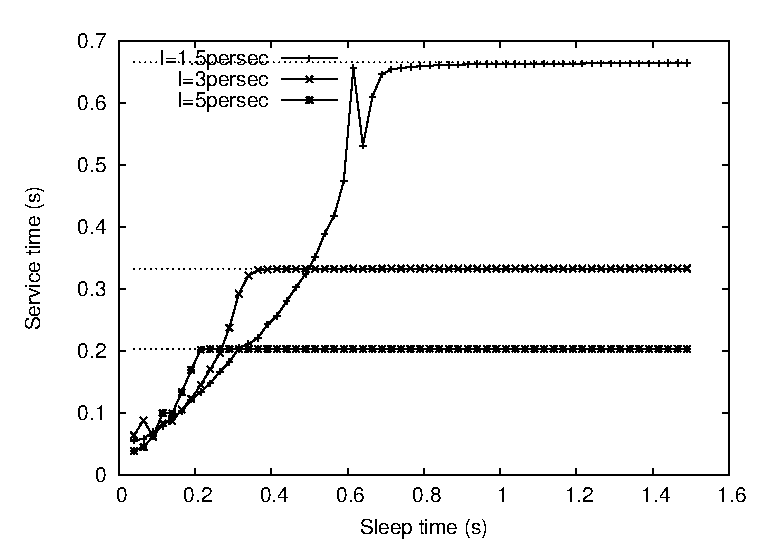
\includegraphics[scale=0.65]{figures/3node_varySleep_sim_x.eps}
\caption{Service time as calculated from the model}
\label{fig:3nodes_x}
\end{figure}

\begin{figure}[t]
\centering
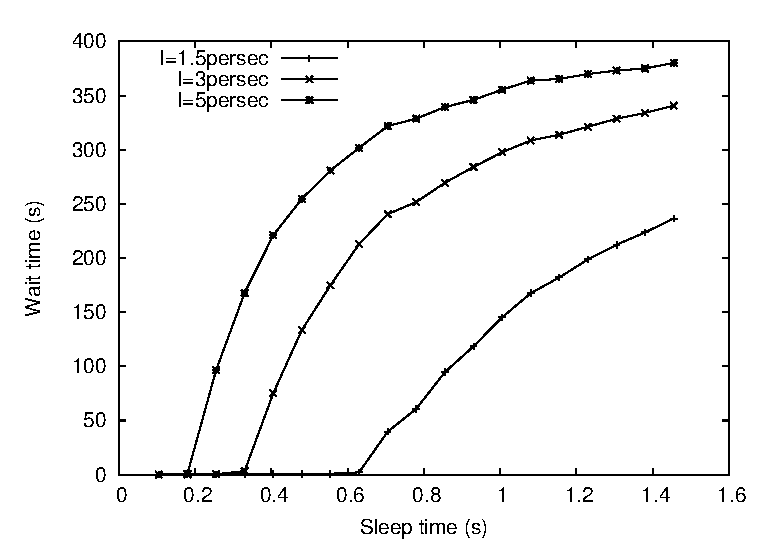
\includegraphics[scale=0.65]{figures/3node_varySleep_sim_large.eps}
\caption{Service time as calculated from the model}
\label{fig:3nodes_large}
\end{figure}

\begin{figure}[t]
\centering
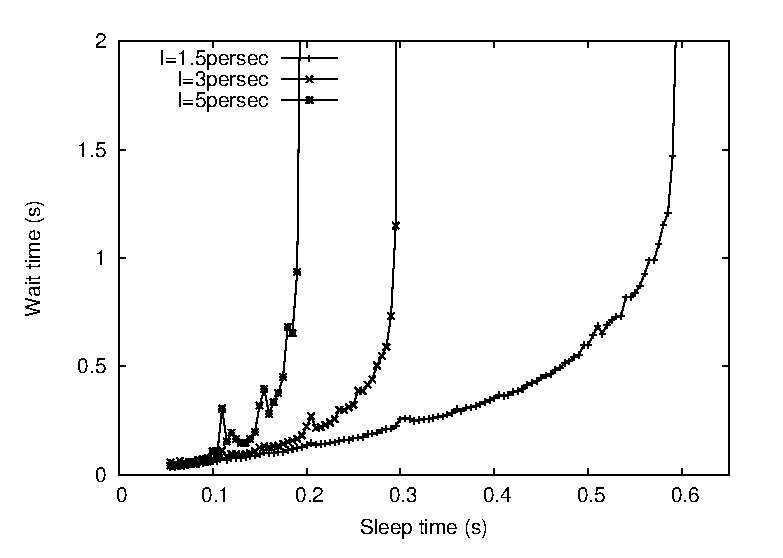
\includegraphics[scale=0.65]{figures/3node_varySleep_sim_small.eps}
\caption{Service time as calculated from the model with non-saturated channel values}
\label{fig:3nodes_small}
\end{figure}

In Figure~\ref{fig:3nodes_x} the service times of a topology with three end nodes are displayed while varying sleeping times. The figure shows results for three different workloads. It is clear from the figure that the service time is upper bounded. The interesting observation is that this upper bound is equal to the inverse of the workload, \emph{i.e.}, the average interarrival time. We call the point where the service time converges as the \emph{saturation point}. Prior to the saturation point, the service time increases proportionally to sleep time. This observation can help us in using our model; for sleeping times smaller than the saturation point we set the value for the service time according to an approximation of a monotonic function. Otherwise, sleeping time is set to be the average interarrival time.

Another observation is that although the service time values are increasing prior to saturation, their effect is not observable until the intensity is approaching 1. This is due the dominanace of the second term in equation~\ref{eq:waiting_2} that corresponds to (\emph{sleeping time}). This is demonstrated in Figures~\ref{fig:3nodes_large} and \ref{fig:3nodes_small}. Prior to the saturation point, the wait times are relatively small and dominated by the sleeping time, as shown in Figure~\ref{fig:3nodes_small}. However, after the saturation point, Figure~\ref{fig:3nodes_large}, the intensity is approaching 1 and therefore causes a dramatic increase in wait times.

\begin{figure}[t]
\centering
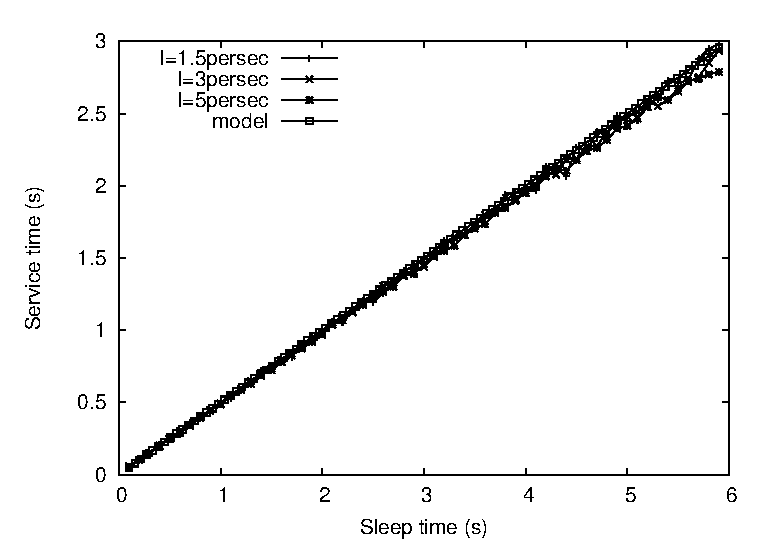
\includegraphics[scale=0.65]{figures/1node_varySleep_sim.eps}
\caption{Sleep times for a network with one end-node compared with the model}
\label{fig:1node}
\end{figure}

\begin{figure}[t]
\centering
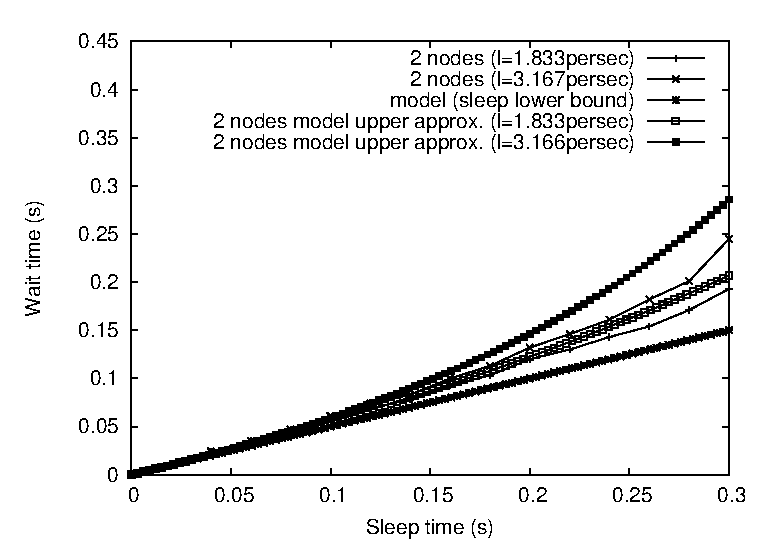
\includegraphics[scale=0.65]{figures/sleep_model_2nodes.eps}
\caption{Comparing wait times for a 2-node network with upper and lower bounds obtained through model}
\label{fig:wait_times_2nodes}
\end{figure}


\subsection{Model validation}
In this section we will demonstrate the behavior of low load scenario; We observe how a small value of service time can make the wait time derivable from the sleeping time only. First, we show a baseline case for a topology with one end-node in Figure~\ref{fig:1node}. In this scenario, the channel does not saturate and the service times are always small, rendering wait times to be dominated by sleep times. Therefore, the different in workloads is not observed and all plots overlap with the model. Now, we show a scenario with two end-nodes and show how the model predict behavior when sleep times approach saturation point. Figure~\ref{fig:wait_times_2nodes} shows these results.

\begin{figure}[t]
\centering
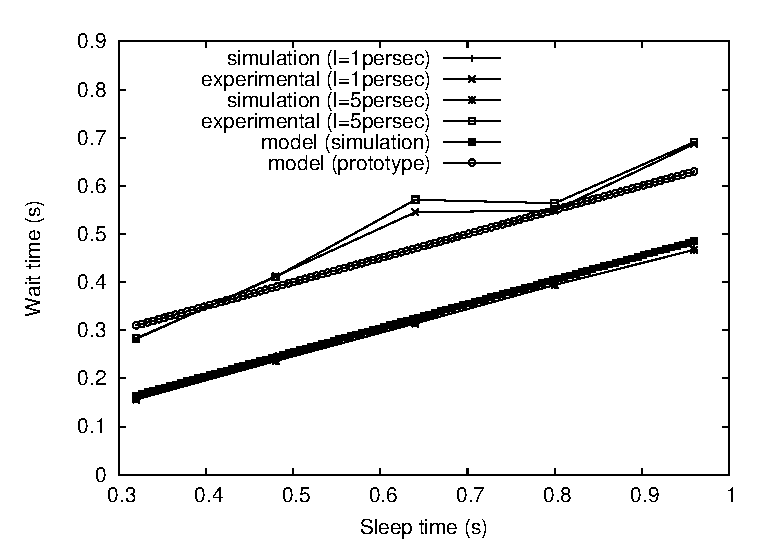
\includegraphics[scale=0.65]{figures/1node_both.eps}
\caption{Comparing wait times of simulation, prototype, and model for a single node network}
\label{fig:1node_both}
\end{figure}

\subsection{prototype evaluation}
Now we will display results obtained from our model to demonstrate its behavior in accordance to our model. In Figure~\ref{fig:1node_both} the results of a single-node prototype is compared to simulation and model. The same behavior is experienced by both node. However, the longer overhead of polling for the prototype makes the wait times larger. 




\subsection{Assigning sleeping times}




